% ============================================
% Evaluación en Dataset Externo Real
% ============================================
\section{Resultados}

% --- Slide 1: Presentación del dataset externo ---
\begin{frame}{Evaluación en Dataset Externo Real}
    \begin{columns}[T]
        \column{0.5\textwidth}

        \begin{block}{Dataset externo}
            Se utilizaron \textbf{24 imágenes SEM reales} (no simuladas) con sus parámetros geométricos medidos manualmente para evaluar la generalización del modelo.
        \end{block}

        \begin{alertblock}{Objetivo}
            Verificar si el modelo entrenado con imágenes simuladas es capaz de predecir correctamente los parámetros de imágenes reales.
        \end{alertblock}

        \begin{exampleblock}{Métrica}
            MAPE sobre $R$, $DCC$ y $P$ en espacio real (unidades originales).
        \end{exampleblock}

        \column{0.5\textwidth}

        \begin{center}
            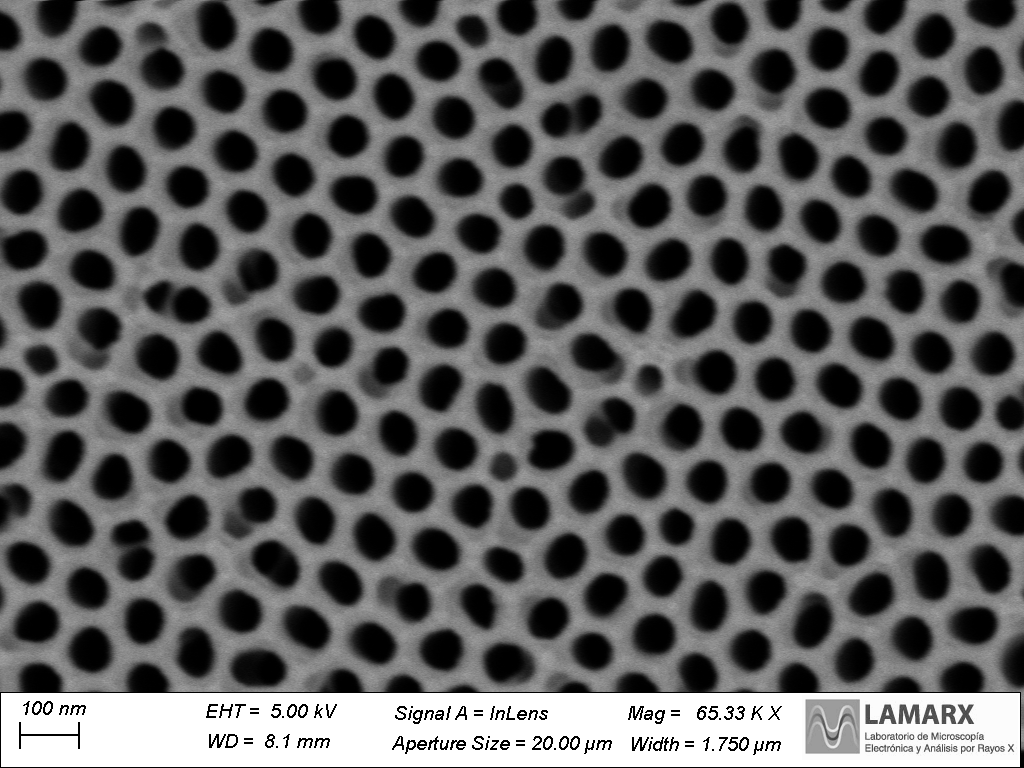
\includegraphics[width=0.9\textwidth]{chapters/Resultados/ImagenSEM.png}

            \small Imagen SEM real con franja de parámetros
        \end{center}

    \end{columns}
\end{frame}

% --- Slide 2: Desafíos, solución y pipeline ---
\begin{frame}{Evaluación en Dataset Externo Real: Pipeline}
    \begin{columns}[T]
        \column{0.5\textwidth}

        \begin{alertblock}{Desafíos de las imágenes SEM reales}
            \begin{enumerate}
                \item Las imágenes tienen resolución mas grande a la utilizada en el entrenamiento.
                \item Las imágenes suelen incluir una franja impresa con parámetros del microscopio (escala, voltaje, etc.).
            \end{enumerate}
        \end{alertblock}

        \begin{block}{Solución: recorte por esquina}
            Para cada imagen se seleccionó una esquina de $300\times300$ px libre de la franja de parámetros del microscopio.
        \end{block}

        \column{0.45\textwidth}

        \begin{exampleblock}{Pipeline de evaluación}
            \small
            \begin{enumerate}
                \item Leer labels en espacio real (sin estandarizar)
                \item Recortar cada imagen a $300\times300$ px sin franja de parámetros
                \item Normalizar píxeles igual que en el entrenamiento
                \item Obtener predicciones y convertirlas al espacio real
                \item Calcular MAPE sobre $R$, $DCC$, $P$
            \end{enumerate}
        \end{exampleblock}

    \end{columns}

    \begin{block}{Nota}
        Los parámetros reales de las imágenes SEM están en unidades originales. Las predicciones del modelo se desnormalizan antes de comparar, para que ambos estén en el mismo espacio.
    \end{block}

\end{frame}

% --- Slide 3: Resultados numéricos ---
\begin{frame}{Evaluación en Dataset Externo Real: Resultados}

    \begin{columns}[T]
        \column{0.30\textwidth}
        \begin{exampleblock}{MAPE — 24 imágenes SEM}
            \renewcommand{\arraystretch}{0.9}
            \begin{tabular}{@{}lc@{}}
            \toprule
            Variable & MAPE \\
            \midrule
            Radio $R$       & $11.00\%$ \\
            Distancia $DCC$ & $11.53\%$ \\
            Porosidad $P$   & $20.51\%$ \\
            \bottomrule
            \end{tabular}
        \end{exampleblock}

        \column{0.6\textwidth}
        \begin{block}{Conclusión}
            El modelo es aceptable: la mayoría de las imágenes presentan errores por debajo del $20\%$.
        \end{block}
    \end{columns}

    \vspace{0.1cm}
    \begin{center}
        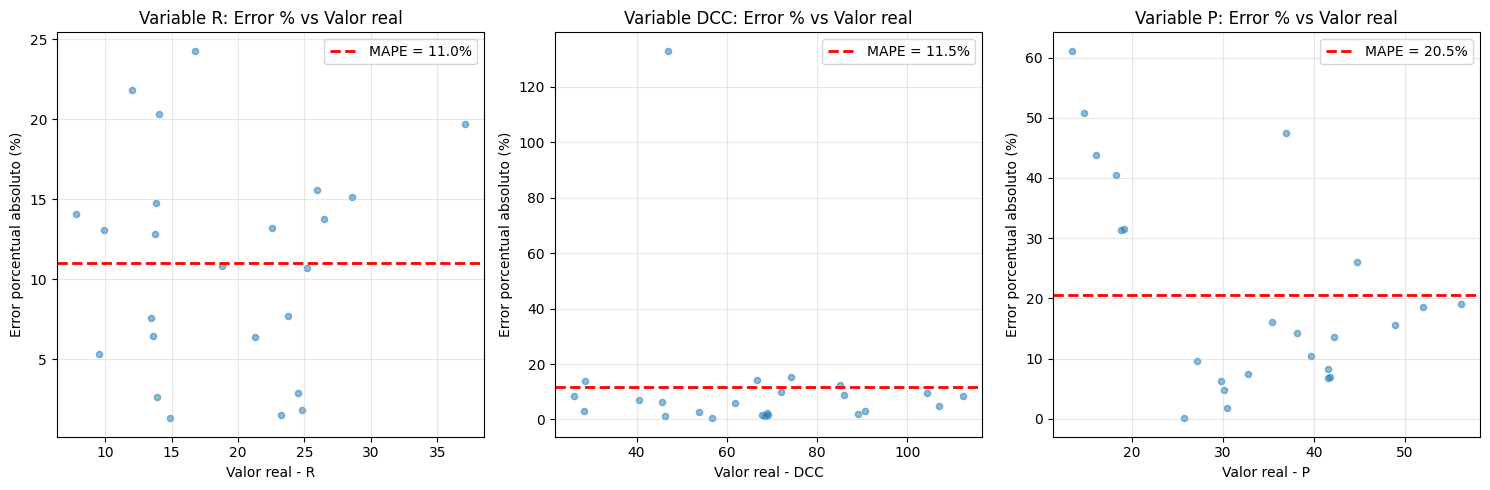
\includegraphics[width=0.8\textwidth]{chapters/Resultados/resultados_conv.png}
    \end{center}

\end{frame}

% ============================================
% DIAPOSITIVA FINAL
% ============================================

\begin{frame}[plain]
    \begin{center}
        {\Large \textbf{¡Gracias!}}
        
    \end{center}
\end{frame}
